% Pipeline teaser (Figure 1) is emitted into the title top matter via
% \pipelineteaser (preamble.tex). Its counter step + label live here in the body
% for pass-stable numbering: teaser pipeline = Fig. 1. The next two body floats
% are declared below so that they print on p.2, next to their first mention in
% the contributions list: fig:setup (Fig. 2) and fig:efficiency (Fig. 3). They
% are discussed in full in Secs. 3 and 5.
\refstepcounter{figure}\label{fig:pipeline}

\section{Introduction}
\label{sec:intro}

Epilepsy affects roughly 1\% of the world's population~\cite{liu2026}. Almost
everything we know about its mechanisms, and every candidate anti-seizure
therapy, is first established in animal models, predominantly chemically or
electrically induced rodents~\cite{bhatt2021}. These studies rest on
\emph{synchronized video--EEG}: an overhead camera records behavior while
implanted electrodes record cortical activity. The two modalities are
complementary. Electrographic seizures can occur with little visible movement,
and movement artifacts routinely corrupt the EEG, so an experimenter confirms
that an event is a seizure, and grades its behavioral severity on the Racine
scale, only by reading both channels together~\cite{racine1972, lundt2015}. This
complementarity makes video--EEG the gold standard of preclinical epilepsy
research~\cite{bhatt2021}.

Manual scoring makes this rigor expensive. A single study can generate thousands
of hours of paired video and EEG, and a trained annotator reviews all of it.
Automating the behavioral half of this workflow is a \emph{video-understanding}
problem: modern action-recognition
backbones~\cite{carreira2017i3d,tran2018r2plus1d,feichtenhofer2019slowfast} and
animal pose estimators~\cite{mathis2018deeplabcut,pereira2022sleap} are mature
and transferable. Yet the epilepsy literature has been slow to adopt them,
especially in animal studies. Video-only rodent detection has only just acquired
its first public benchmark~\cite{rodepil2025}, and computational video--EEG
fusion in animals is confined to two isolated \emph{binary}
detectors~\cite{mullen2024,eegvfusion2026}, neither grading severity. No one has yet measured \emph{how far standard video deep learning actually gets}
on this problem against a strong EEG reference on the same data.

% --- p.2 floats: acquisition, one synchronized pair, and the headline
% efficiency result. Declared here (rather than in Secs. 3-5, where each is
% discussed) so they print beside their first mention in the contributions list.
\begin{figure}[t]
\centering
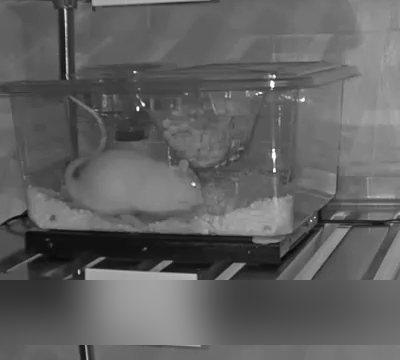
\includegraphics[width=0.60\linewidth]{fig/stages/f_setup.png}
\caption{A representative overhead frame of the acquisition setup: each rat is
recorded in its home cage by a fixed overhead camera while implanted electrodes
stream synchronized EEG, and the cage rests on a per-animal platform. Camera
geometry differs per cage, so clips are per-cage cropped before subjects are
pooled. De-identified (cage-side identifier redacted).}
\label{fig:setup}
\end{figure}

% fig:paired now lives in sec/2_related.tex so it prints on the Related Work page
% beside the multimodal video--EEG paragraph it illustrates.

\begin{figure}[t]
\centering
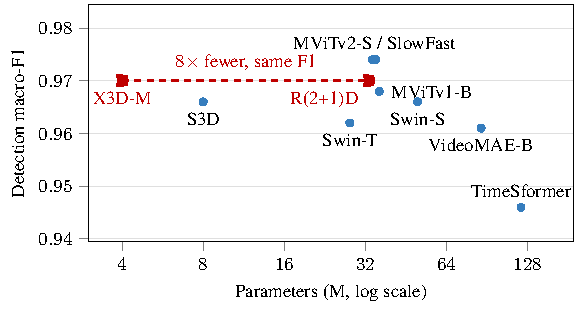
\includegraphics[width=\linewidth]{fig/fig_efficiency.pdf}
\caption{Detection accuracy \vs\ model size across ten video backbones (accuracies from
Table~\ref{tab:vidarch}, parameter counts from Table~\ref{tab:vidspec}). Every
architecture lands in a narrow 0.946--0.974 macro-F1 band, and the 4M-parameter
X3D-M ties the 33M R(2+1)D-18 at 0.970, an $8\times$ saving at no cost in
accuracy.}
\label{fig:efficiency}
\end{figure}

This paper provides that account. The contribution is empirical: on a real
preclinical cohort, under a single controlled protocol, we report where a standard video backbone matches EEG,
where it surpasses it, where it breaks, and how the choice of architecture,
temporal sampling, data budget and evaluation protocol shape the answer. A
comprehensive literature survey of the field (video-only and multimodal
video--EEG detection across human and animal subjects) is provided in the
supplementary material (App.~\ref{sec:survey}); the main paper is the empirical
study.

We organize that study around four questions:
\begin{itemize}[leftmargin=2.6em,itemsep=1pt,topsep=2pt]
  \item[\textbf{RQ1}] \emph{What model and input capacity is sufficient?}
  (Sec.~\ref{sec:rq1})
  \item[\textbf{RQ2}] \emph{Do the two modalities fail in the same way, or are
  their errors complementary?} (Sec.~\ref{sec:crossmodal})
  \item[\textbf{RQ3}] \emph{Once a seizure is identified, does ordinal modeling
  improve Stage\,2--5 grading and reduce large-stage errors on unseen subjects?}
  (Sec.~\ref{sec:problem:ordinal})
  \item[\textbf{RQ4}] \emph{Does inverse-frequency weighting keep the long tail
  from dominating the result?} (Sec.~\ref{sec:rq3})
\end{itemize}
All four rest on the head-to-head comparison itself: how far a standard
video backbone gets against an electrode-based reference, and whether that ordering
survives held-out animals and an external benchmark
(Sec.~\ref{sec:crossmodal}). Our contributions are:

\begin{itemize}
  \itemsep0.15em
  \item A \textbf{pooled twenty-subject synchronized video--EEG cohort}
  (Sec.~\ref{sec:data}): $\sim$24k expert-annotated, per-cage-cropped clips over
  601 sessions with per-clip Racine severity labels and severely long-tailed
  burden. To our knowledge this is the largest paired rodent video--EEG corpus
  studied for learned detection. Figure~\ref{fig:setup} shows the acquisition setup: one
  fixed overhead camera per home cage, so geometry is constant within an animal and
  differs across animals, which is why we crop per cage. We release a fully
  de-identified description.
  \item A \textbf{head-to-head video-\vs-EEG comparison} across three task
  granularities (Sec.~\ref{sec:application}) under a matched, leakage-controlled
  protocol. Video matches a strong EEG reference on detection (0.993 \vs\ 0.992
  AUROC) and degrades far more gracefully on severity grading, with Grad-CAM
  evidence that the model attends to behaviorally meaningful regions.
  \item A \textbf{controlled sweep of ten video backbones and seven EEG models},
  plus temporal-sampling, resolution, data-efficiency and pretraining ablations.
  Detection is backbone-agnostic on this cohort (Fig.~\ref{fig:efficiency}):
  accuracy is flat in model size, and a 4M-parameter X3D matches a 33M R(2+1)D.
  Temporal context is what matters: a single-frame control collapses at
  every granularity (0.569 macro-F1 at detection against 0.970 at 16 frames),
  which shows the task is read from motion. Under \textbf{subject-disjoint}
  cross-validation the two modalities stay level at detection, while video's
  advantage at 3- and 5-class grading holds.
  \item \textbf{External validation} on the public RodEpil
  benchmark~\cite{rodepil2025} (0.979 subject-wise F1), together with a
  documented encoding artifact in its raw release that must be corrected for an
  honest score.
\end{itemize}
